\section{Исследовательская часть}

В данном разделе будет исследован процесс утверждения темы. Модель бизнес-процесса представлена на рисунке \ref{fig:vkrbpmn}.

\begin{figure}[h!btp]
	\centering
	\includegraphics[width=\textwidth]{inc/vkr\_bpmn.pdf}
	\caption{Модель сети Петри}
	\label{fig:vkrbpmn}	
\end{figure}

\subsection{Моделирование с помощью sTPN}

Построим соответствующую процессу стохастическую модель сети Петри для дальнейшего моделирования процесса. Итоговая модель сети Петри представлена на рисунке \ref{fig:tpn}.

\begin{figure}[h!btp]
	\centering
	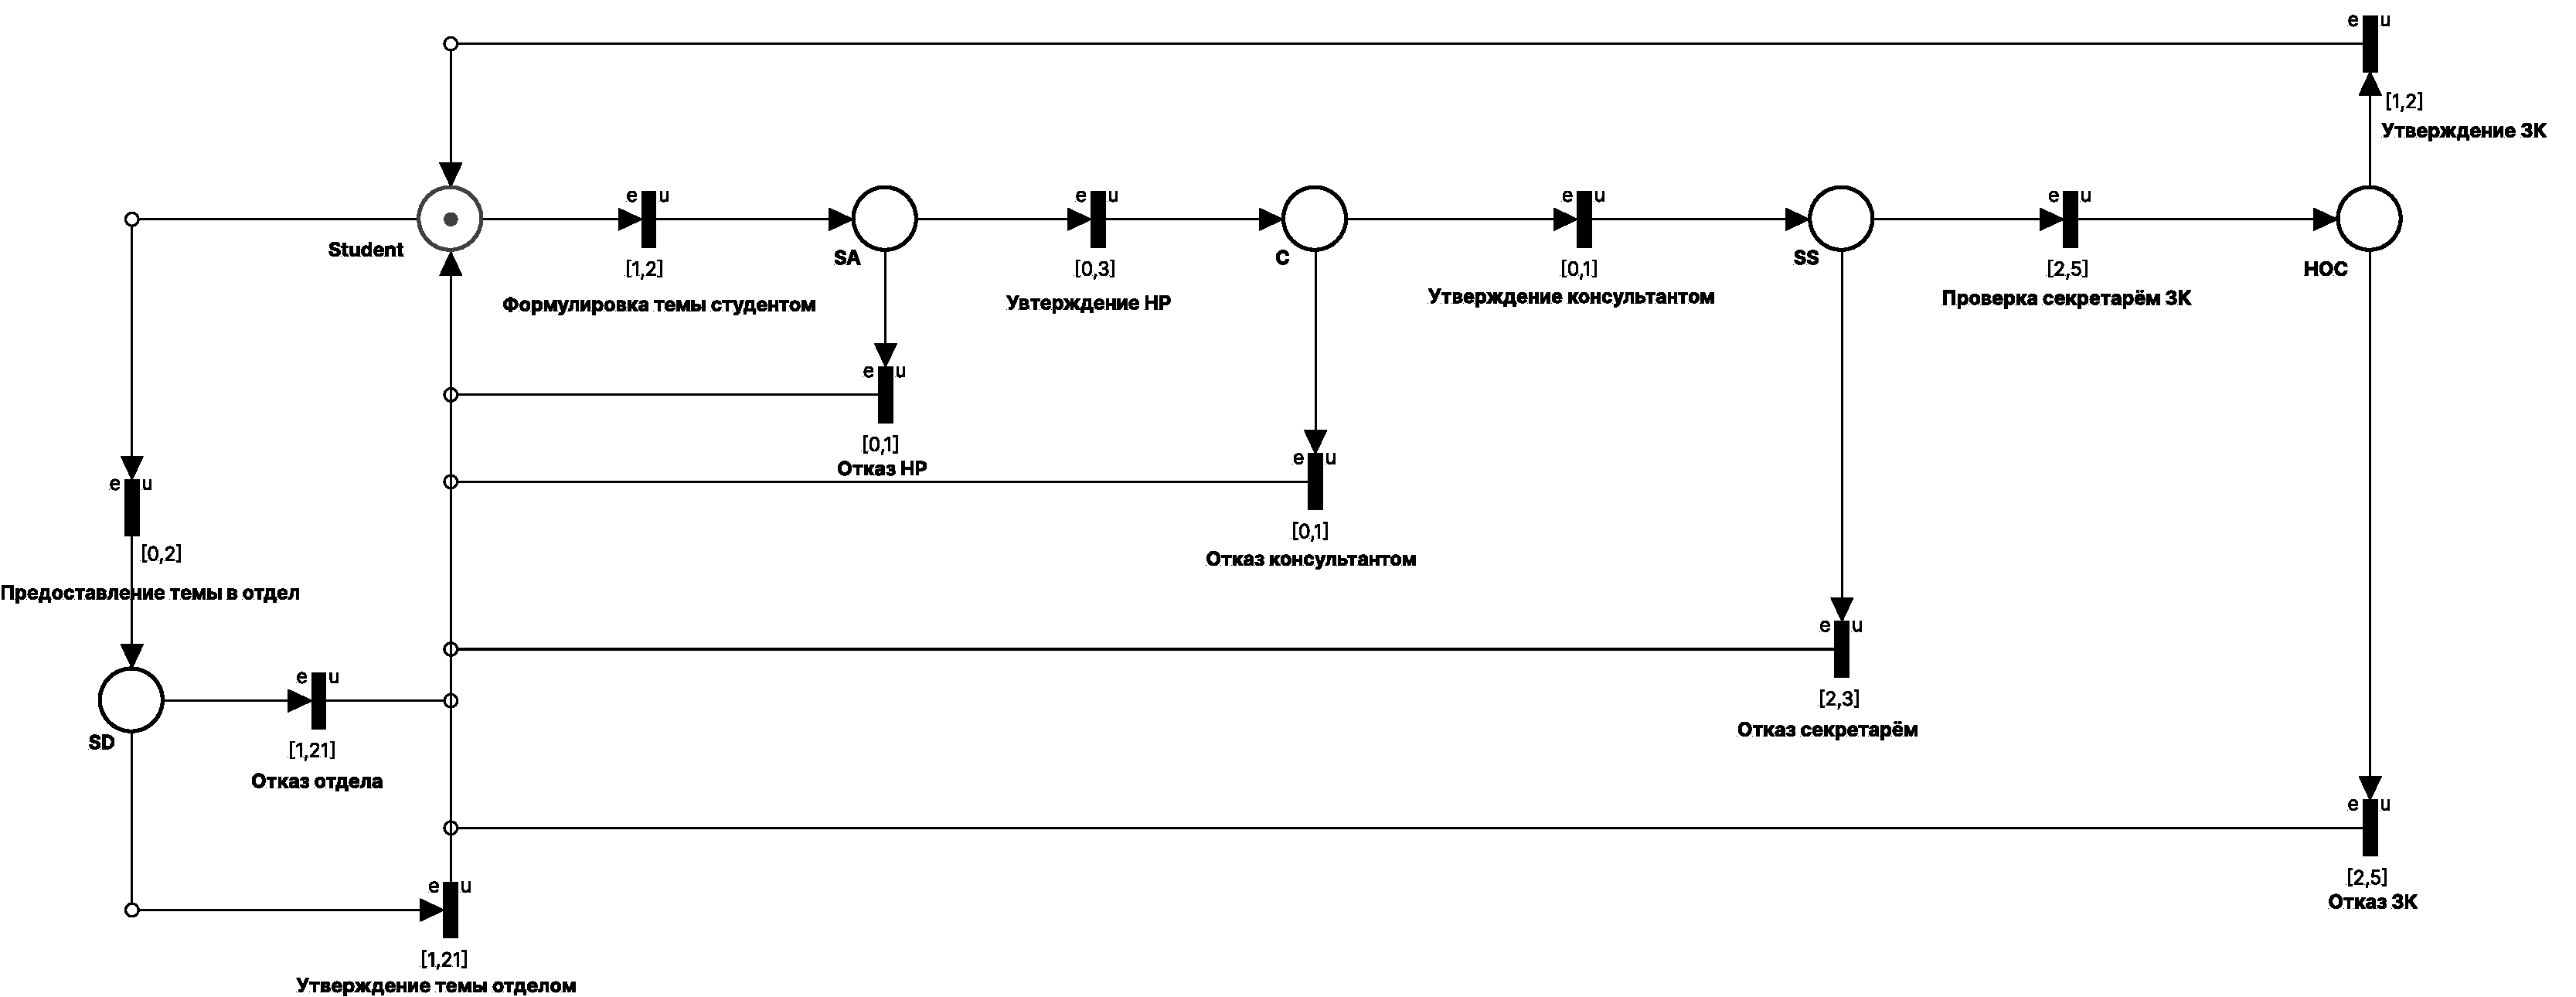
\includegraphics[width=\textwidth]{inc/timed.pdf}
	\caption{Модель сети Петри}
	\label{fig:tpn}	
\end{figure}

Прямой анализ переходных процессов\cite{forward-transient} на временном отрезке в 22 временных единицы показал сходимость модели к 20 временным единицам. Результат прямого анализа переходных процессов представлен на рисунке \ref{fig:ft}.

\clearpage

\begin{sidewaysfigure}[h!btp]
	\centering
	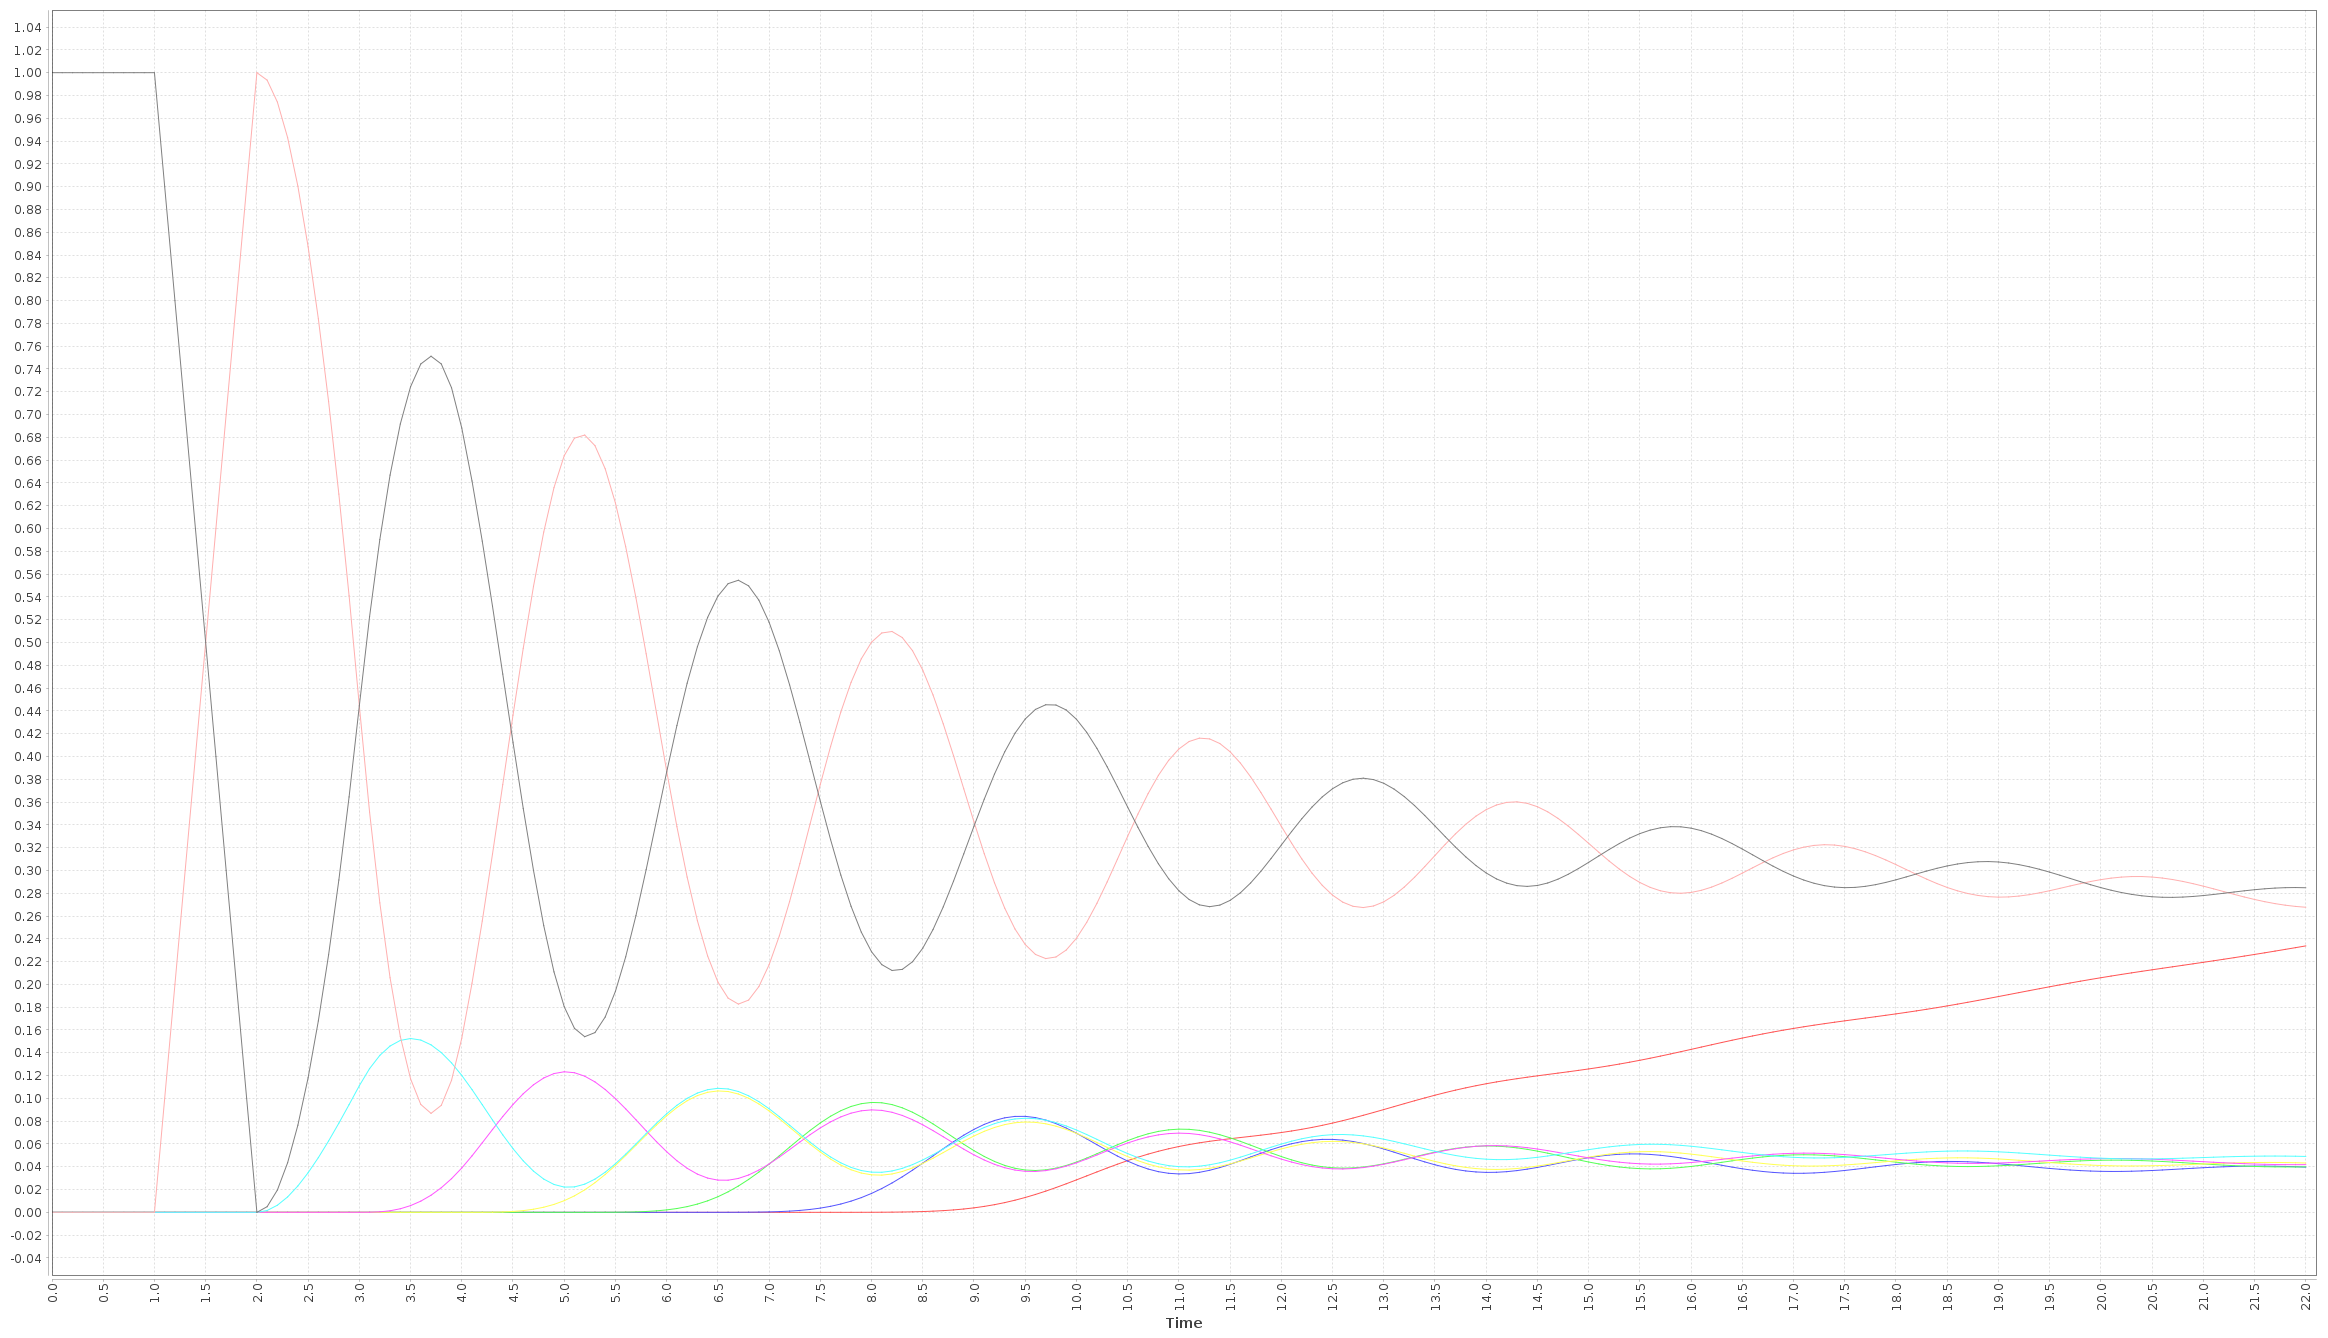
\includegraphics[width=\textwidth]{inc/forward_transient.png}
	\caption{Результат прямого анализа переходных процессов сети Петри}
	\label{fig:ft}
\end{sidewaysfigure}

\clearpage

Регенеративный анализ переходных процессов\cite{regenerative-transient} на временном отрезке в 34 временные единицы с использованием переменной, отвечающей за полное выполнение цикла модели -- \texttt{Reward variable}\cite{reward} подтвердил результаты прямого анализа. Результат регенеративного анализа переходных процессов представлен на рисунке \ref{fig:rt}.

\clearpage

\begin{sidewaysfigure}[h!btp]
	\centering
	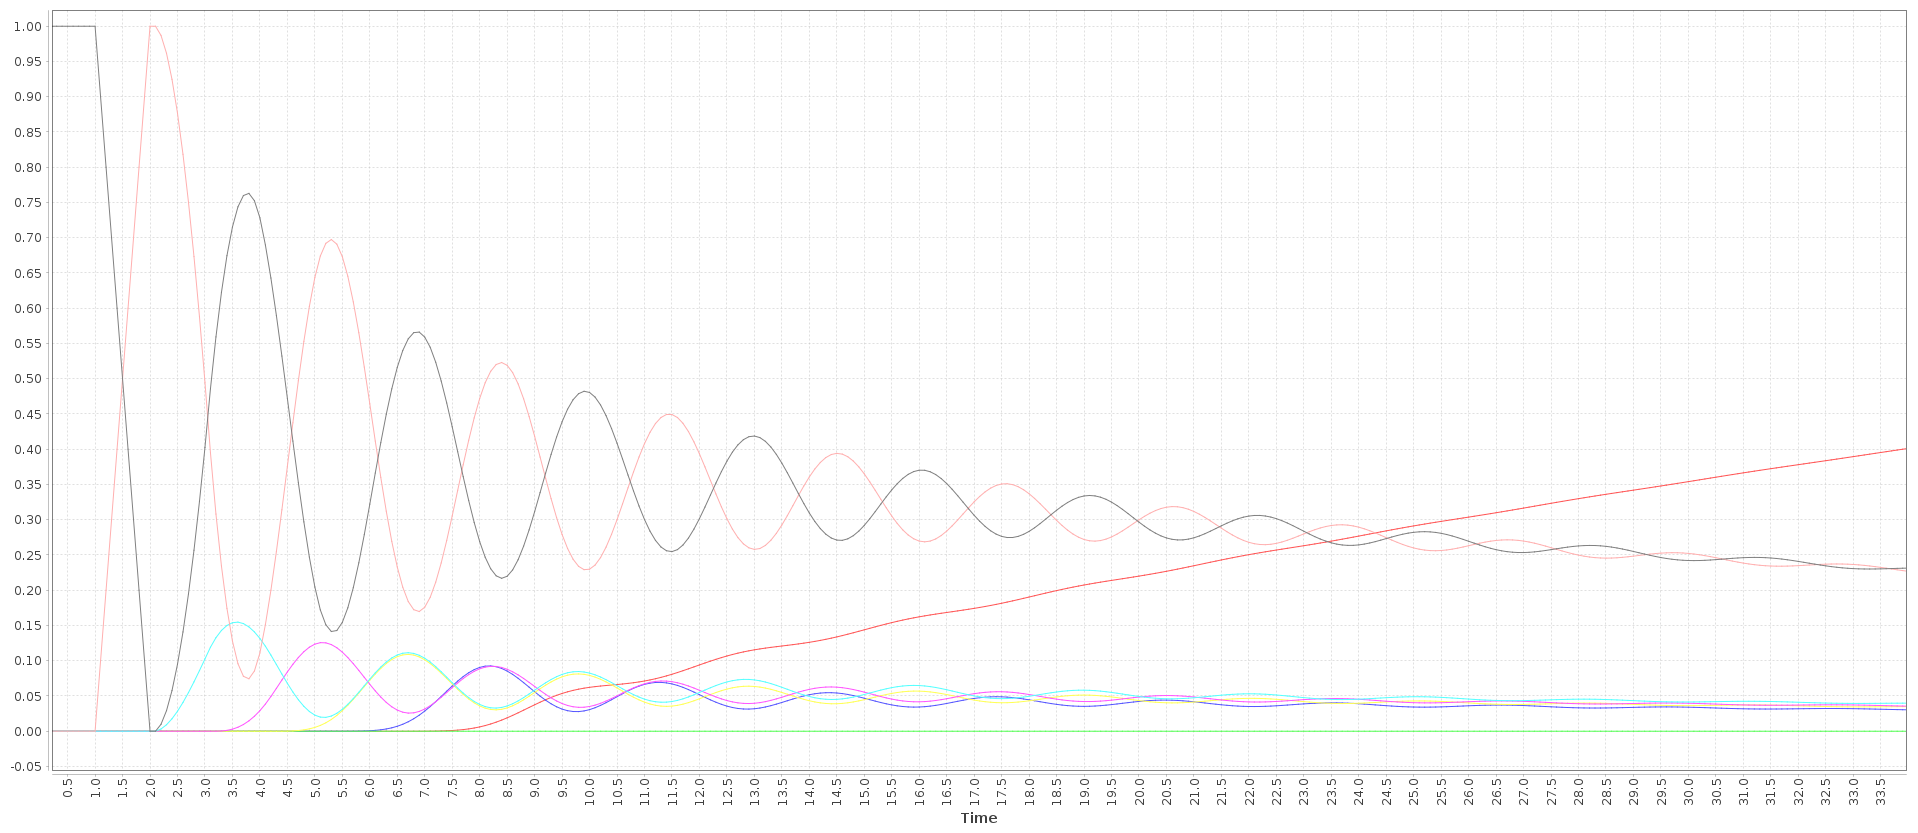
\includegraphics[width=\textwidth]{inc/timed_reward.png}
	\caption{Результат регенеративного анализа переходных процессов}
	\label{fig:rt}
\end{sidewaysfigure}

\clearpage

Результаты заключительного регенеративного анализа для установления отношения вероятности достижения успешного исхода событий от времени представлены на рисунке \ref{fig:sp}.

\begin{figure}[h!btp]
	\centering
	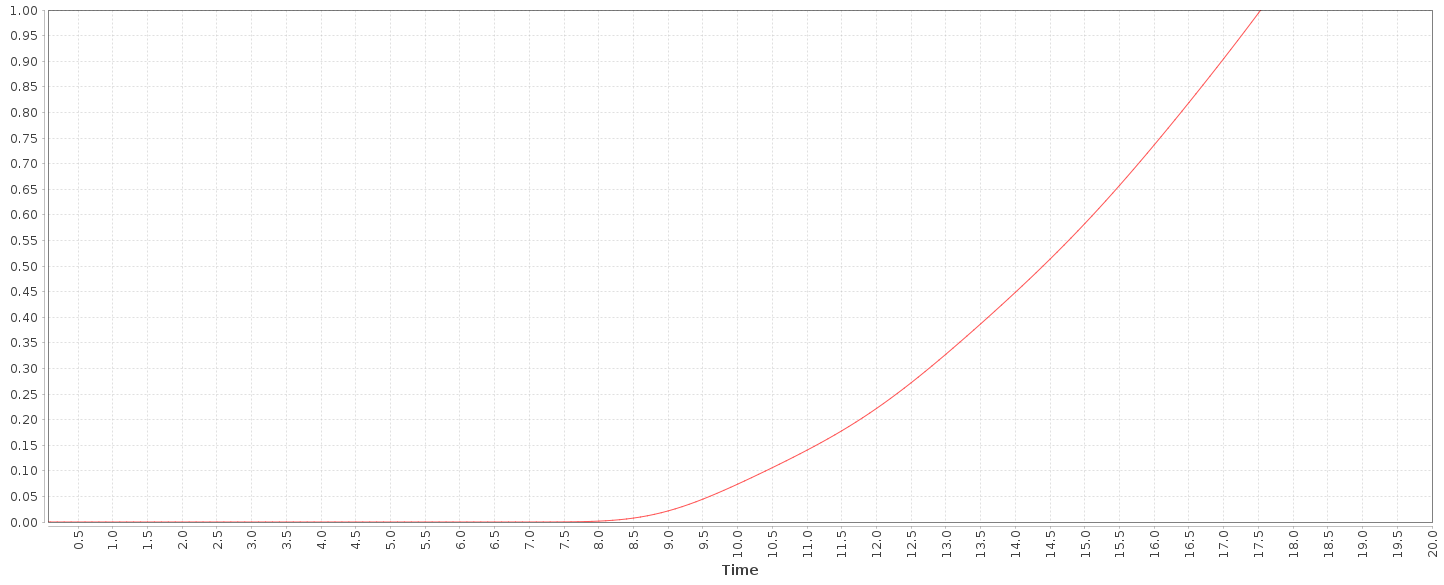
\includegraphics[width=0.9\textwidth]{inc/stud_prob.png}
	\caption{Результат регенеративного анализа сети Петри с переменной}
	\label{fig:sp}
\end{figure}

Исходя из полученных данных прямого и обратного анализов максимальное время на выполнение процесса может занять до 18 временных единиц. Совокупное время моделирования составило 72 часа.

\subsection{Квантовое моделирование}

Для расчёта необходимо заполнить базу знаний. В качестве стохастических переходов использовано аналогичное сетям Петри нормальное распределение с параметрами \texttt{EFT} (\texttt{Expected Finish Time}) и \texttt{LFT} (\texttt{Latest Finish Time}). База знаний представлена на рисунке \ref{fig:knowledge}.

\begin{figure}[h!btp]
	\centering
	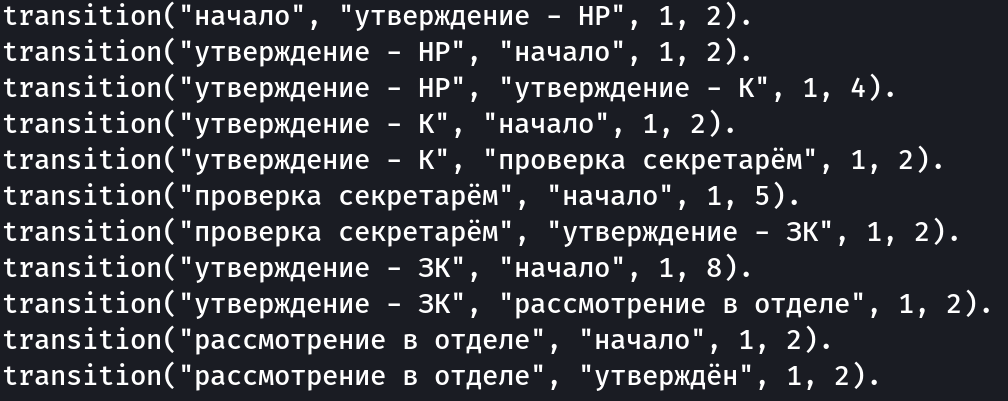
\includegraphics[width=0.9\textwidth]{inc/knowledge.png}
	\caption{База знаний}
	\label{fig:knowledge}
\end{figure}

\pagebreak

%\begin{adjustwidth}{-0.2pt}{0pt}
Результат работы программы представлен на рисунке \ref{fig:res}.
%\end{adjustwidth}

\begin{figure}[h!]
	\centering
	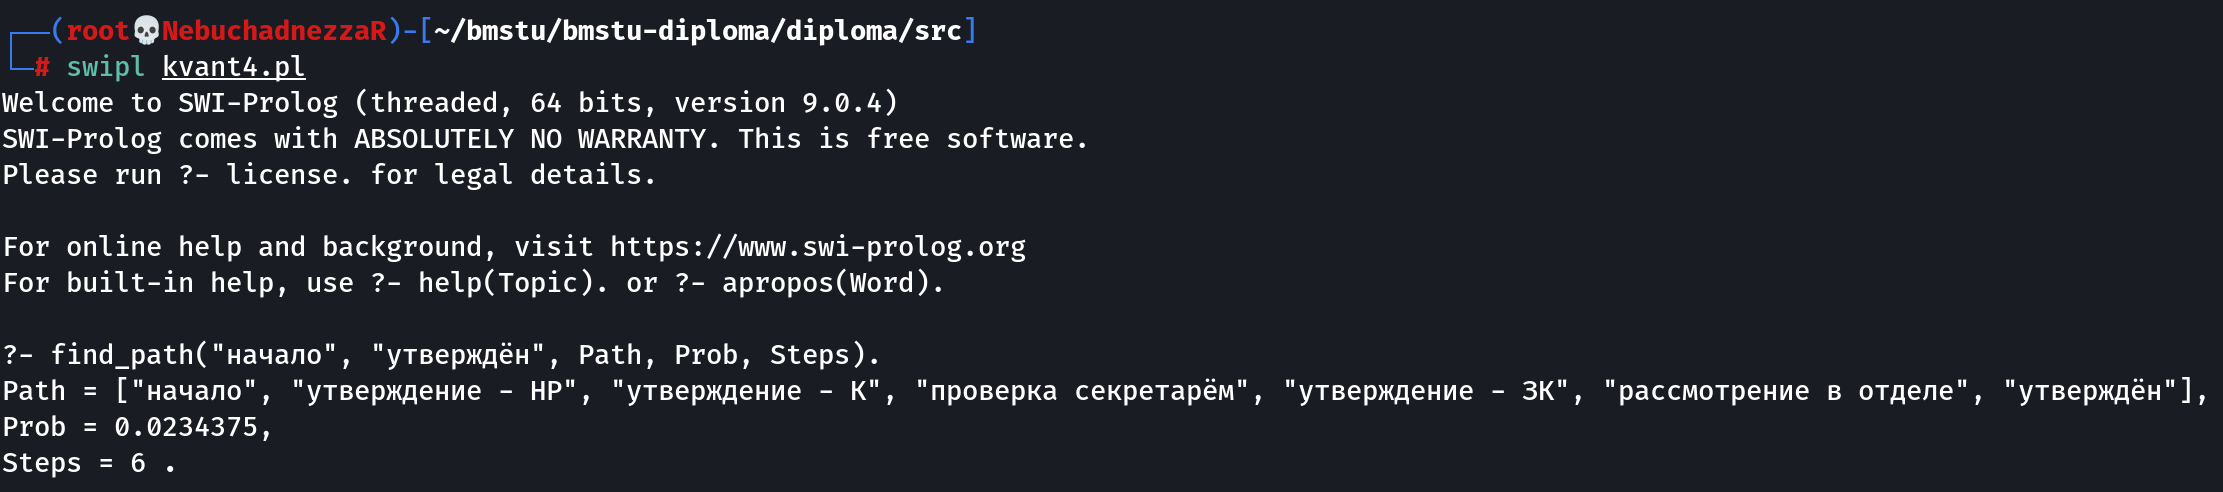
\includegraphics[width=\textwidth]{inc/res.png}
	\caption{Результат работы программы}
	\label{fig:res}
\end{figure}

Вероятность успешно пройти всю цепочку составляет 2.3\%. Распределения вероятностей представлено в таблице \hyperref[tab:distrib]{1} в приложении \hyperref[app:table]{А}. Визуализация полученный данных представлена на рисунке \ref{plt:time}. Совокупное время моделирование составило 2 миллисекунды.

\begin{figure}[h!]
	\centering
	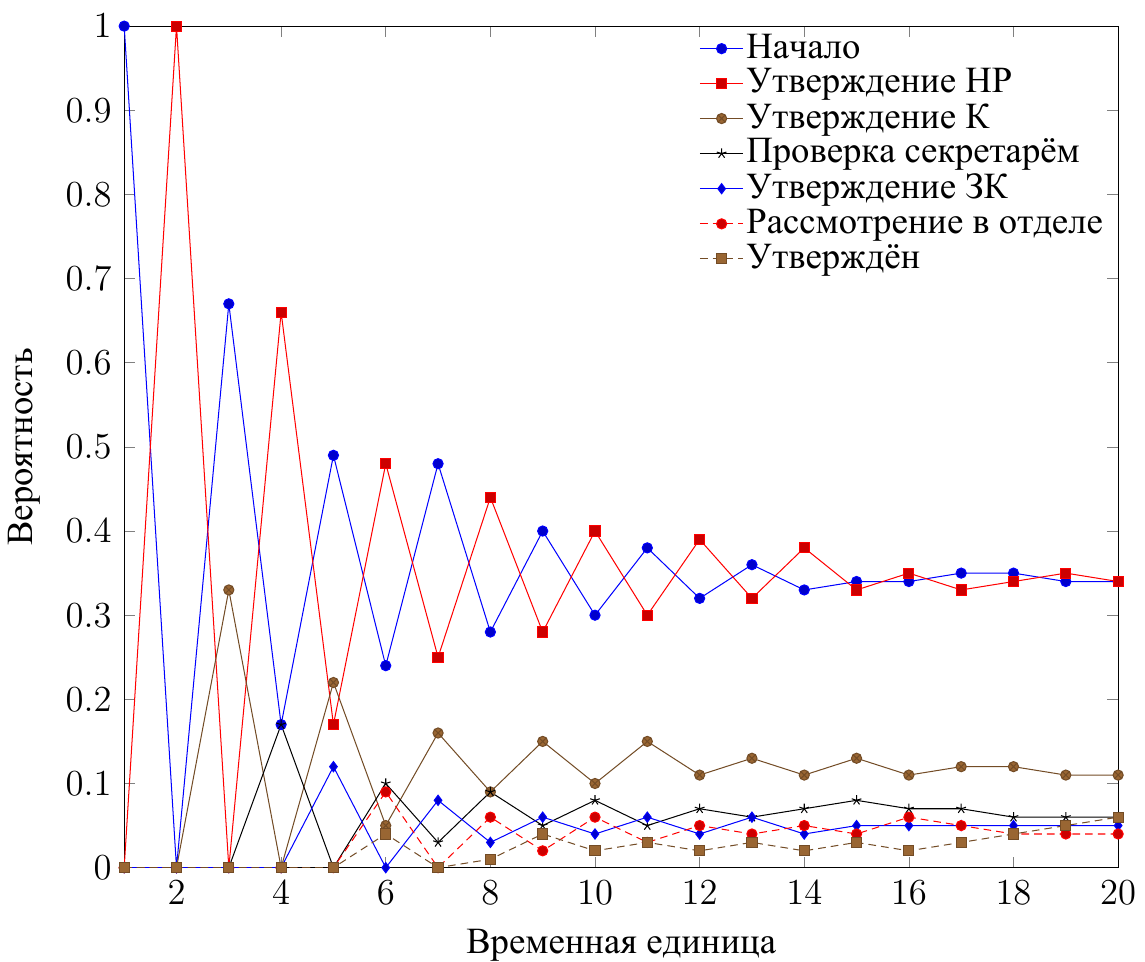
\includegraphics[width=\textwidth]{inc/graph.png}
	\caption{График распределения вероятностей квантового моделирования}
	\label{plt:time}
\end{figure}

%\begin{figure}[h!]
%	\centering
 %   \resizebox{\textwidth}{!}{%
%	\begin{tikzpicture}
%		\begin{axis}[
%			xmin=1, xmax=20, xlabel={Временная единица},
%			ymin=-0, ymax=1, ylabel={Вероятность},
%			legend style={draw=none, fill=none, inner ysep=0pt, outer sep=2pt, nodes={inner sep=1pt}, at={(1,1)}, anchor=north east},
%			legend cell align=left,        
%			]
%			\addplot table [y index=1] {inc/data.txt};
%			\addlegendentry{Начало};
%			\addplot table [y index=2] {inc/data.txt};
%			\addlegendentry{Утверждение НР};
%			\addplot table [y index=3] {inc/data.txt};
%			\addlegendentry{Утверждение К};
%			\addplot table [y index=4] {inc/data.txt};
%			\addlegendentry{Проверка секретарём};
%			\addplot table [y index=5] {inc/data.txt};
%			\addlegendentry{Утверждение ЗК};
%			\addplot table [y index=6] {inc/data.txt};
%			\addlegendentry{Рассмотрение в отделе};
%			\addplot table [y index=7] {inc/data.txt};
%			\addlegendentry{Утверждён};
%		\end{axis}
%	\end{tikzpicture}%
%	}
%	\caption{График распределения вероятностей}
%	\label{plt:time}
%\end{figure}

Возьмём другой произвольный пример. Соответствующая модель представлена на рисунке \ref{fig:test}.

\begin{figure}[h!btp]
	\centering
	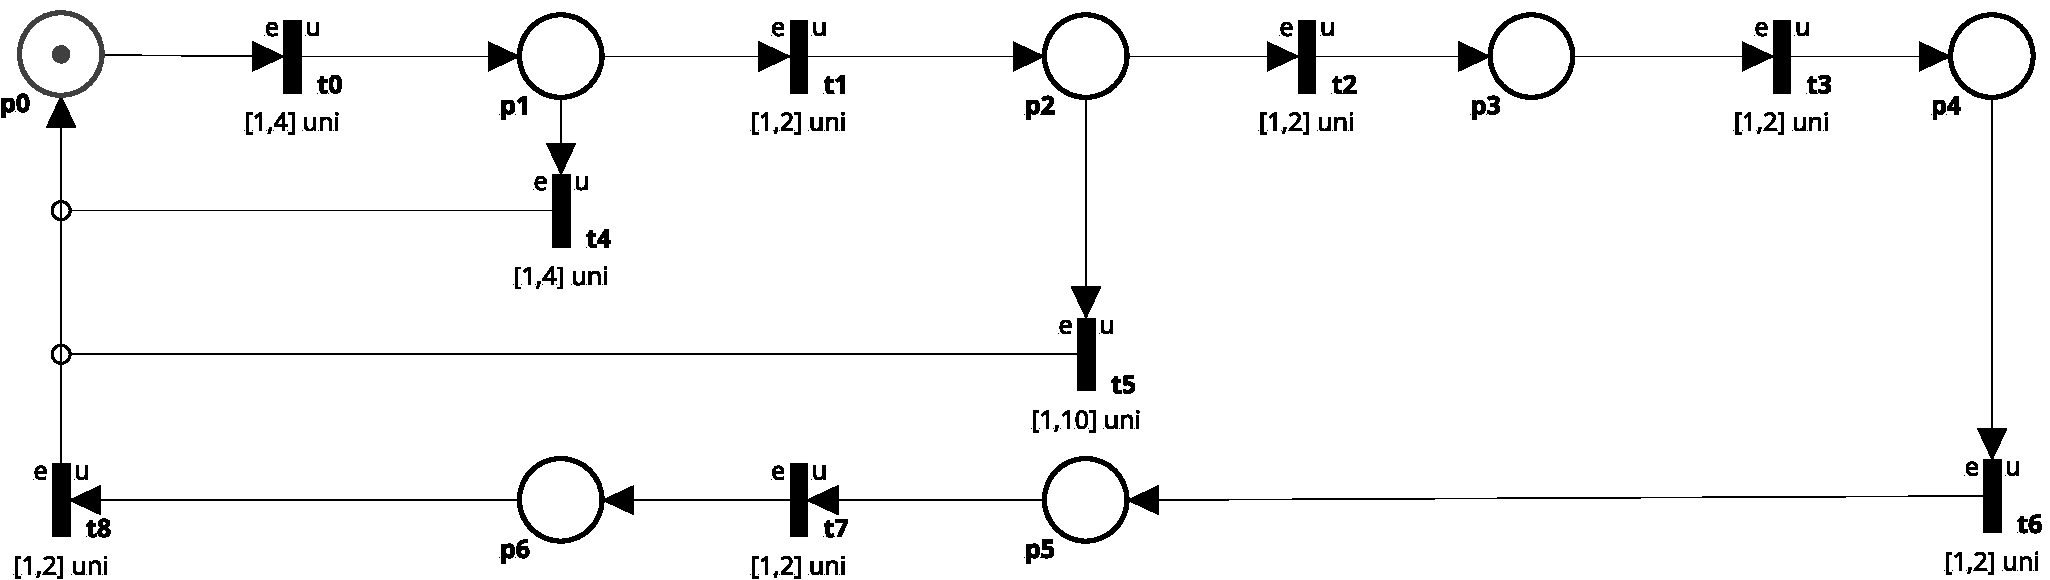
\includegraphics[width=0.8\textwidth]{inc/test.pdf}
	\caption{Модель сети Петри}
	\label{fig:test}	
\end{figure}

Соответствующая база знаний представлена на рисунке \ref{fig:testbz}.

\begin{figure}[h!btp]
	\centering
	\includegraphics[width=0.6\textwidth]{inc/test\_bz.png}
	\caption{База знаний}
	\label{fig:testbz}
\end{figure}

Регенеративный анализ сети Петри представлен на рисунке \ref{fig:testreg}.

\clearpage

\begin{sidewaysfigure}[h!btp]
	\centering
	\includegraphics[width=\textwidth]{inc/test\_reg.png}
	\caption{Результат регенеративного анализа сети Петри}
	\label{fig:testreg}
\end{sidewaysfigure}

\clearpage

Результат моделирования методом квантовых шахмат представлен на рисунке \ref{fig:testchess}.

\begin{figure}[h!btp]
	\centering
	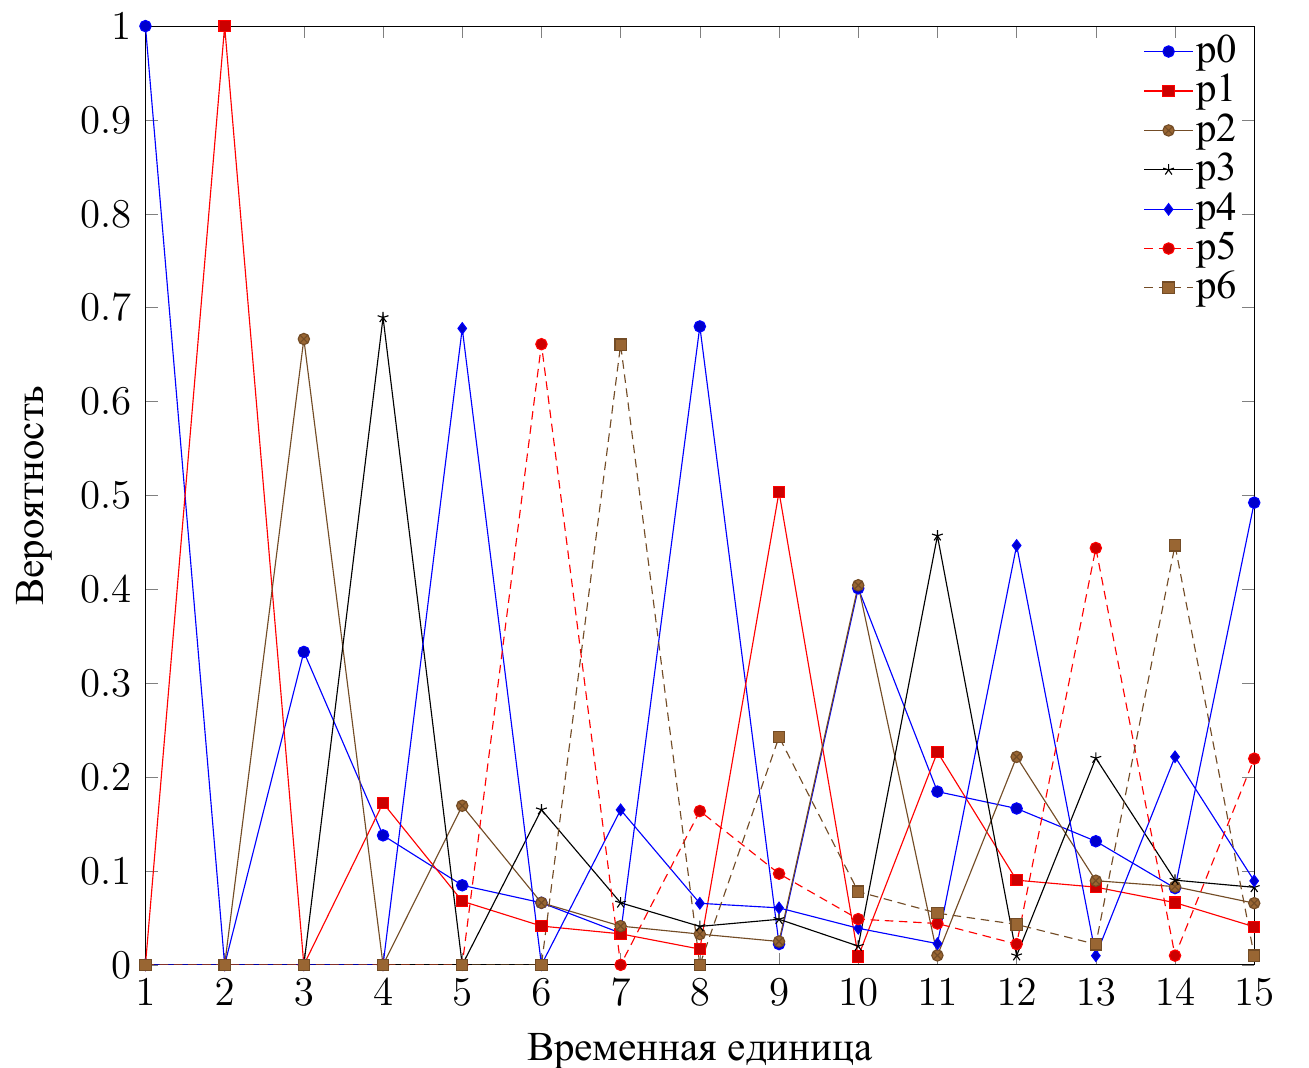
\includegraphics[width=0.75\textwidth]{inc/test.png}
	\caption{Распределение вероятностей моделирования методом квантовых шахмат}
	\label{fig:testchess}
\end{figure}

Исходя из результатов, моделирование методом сетей Петри более точно отражает распределение вероятностей. Методу квантовых шахмат нужно на 20\% больше шагов, чтобы сравняться с сетями Петри, что компенсируется более быстрым расчётом.

\subsection{Вывод}

Анализ данных показал, что максимальное время выполнения процесса может достигать 18 временных единиц, при этом вероятность успешного прохождения всей цепочки составляет 2.3\%.

Квантовое моделирование продемонстрировало практически идентичные результаты распределения вероятностей по сравнению с моделированием с помощью сетей Петри. Однако, квантовое моделирование позволяет получить эти результаты в многократно быстрее, несмотря на невозможность отслеживания пути до конкретного статуса.

Результаты квантового моделирования также показали, что вероятность нахождения в финальном статусе возрастает с каждой итерацией, что подтверждается регенеративным анализом сетей Петри.

\clearpage